\chapter{Methodology}
This chapter covers the various methodologies that were implemented in this 
project. It takes a look at the different types of research methodologies that 
were used such as Qualitative Research, Quantitative Research, and Mixed Methods
Research and the different types of software development methodologies that were
used such as Test Driven Development, Continuous Delivery, Extreme Programming, 
etc. and why each was chosen. Other areas also covered in this chapter include
meetings, project management, development tools, source control, and testing.

\section{Research Methodology}
The research methodology that was used in this project was a Mixed Methods 
Research methodology, using a mix of both Qualitative Research and Quantitative 
Research. Qualitative research approaches are employed across many academic 
disciplines and is useful at an individual level. Qualitative data collection
methods vary using unstructured or semi-structured techniques.
\par
\medskip
Research for this project included looking at and researching how to build a sorting algorithms visualizer \cite{sortal_build} and researching similar applications, such as VisuAlgo, Sorting Visualizer by Clement Mihailescu, and Comparison Sorting Visualization hosted by University of San Francisco. 

\newpage
\subsection{VisuAlgo}
\begin{center}
    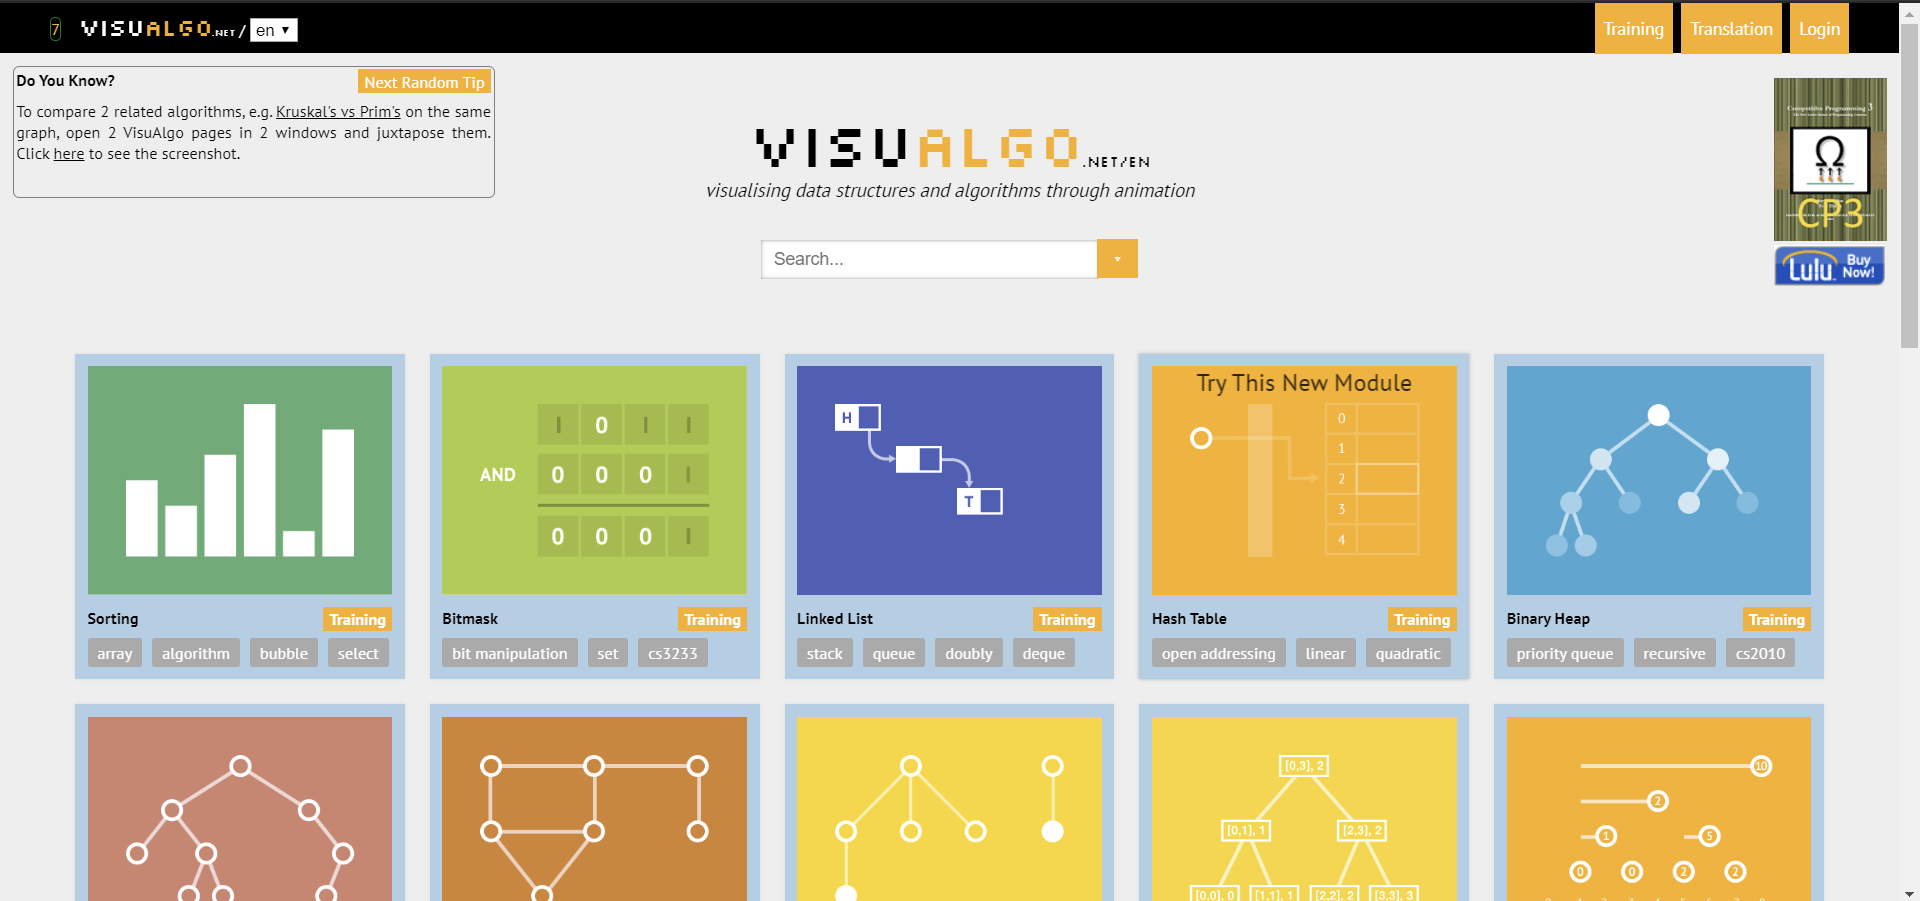
\includegraphics[width=12cm,height=12cm,keepaspectratio]{images/visualgonet}
\end{center}
VisuAlgo \cite{sorting_2} was conceptualised in 2011 by Dr Steven Halim as a tool to help his students better understand data structures and algorithms, by allowing them to learn the basics on their own and at their own pace. VisuAlgo contains many advanced algorithms that are discussed in Dr Steven Halim's book ('Competitive Programming', co-authored with his brother Dr Felix Halim) and beyond. Today, some of these advanced algorithms visualization/animation can only be found in VisuAlgo. VisuAlgo is an ongoing project and more complex visualisations are still being developed.
\par
\bigskip
VisuAlgo contains animations and visualizations for many different algorithms and concepts in Computer Science such as sorting algorithms, linked lists, hash tables, graph traversals, etc. Inspiration for this application was taken from the sorting component of VisuAlgo.
\begin{center}
    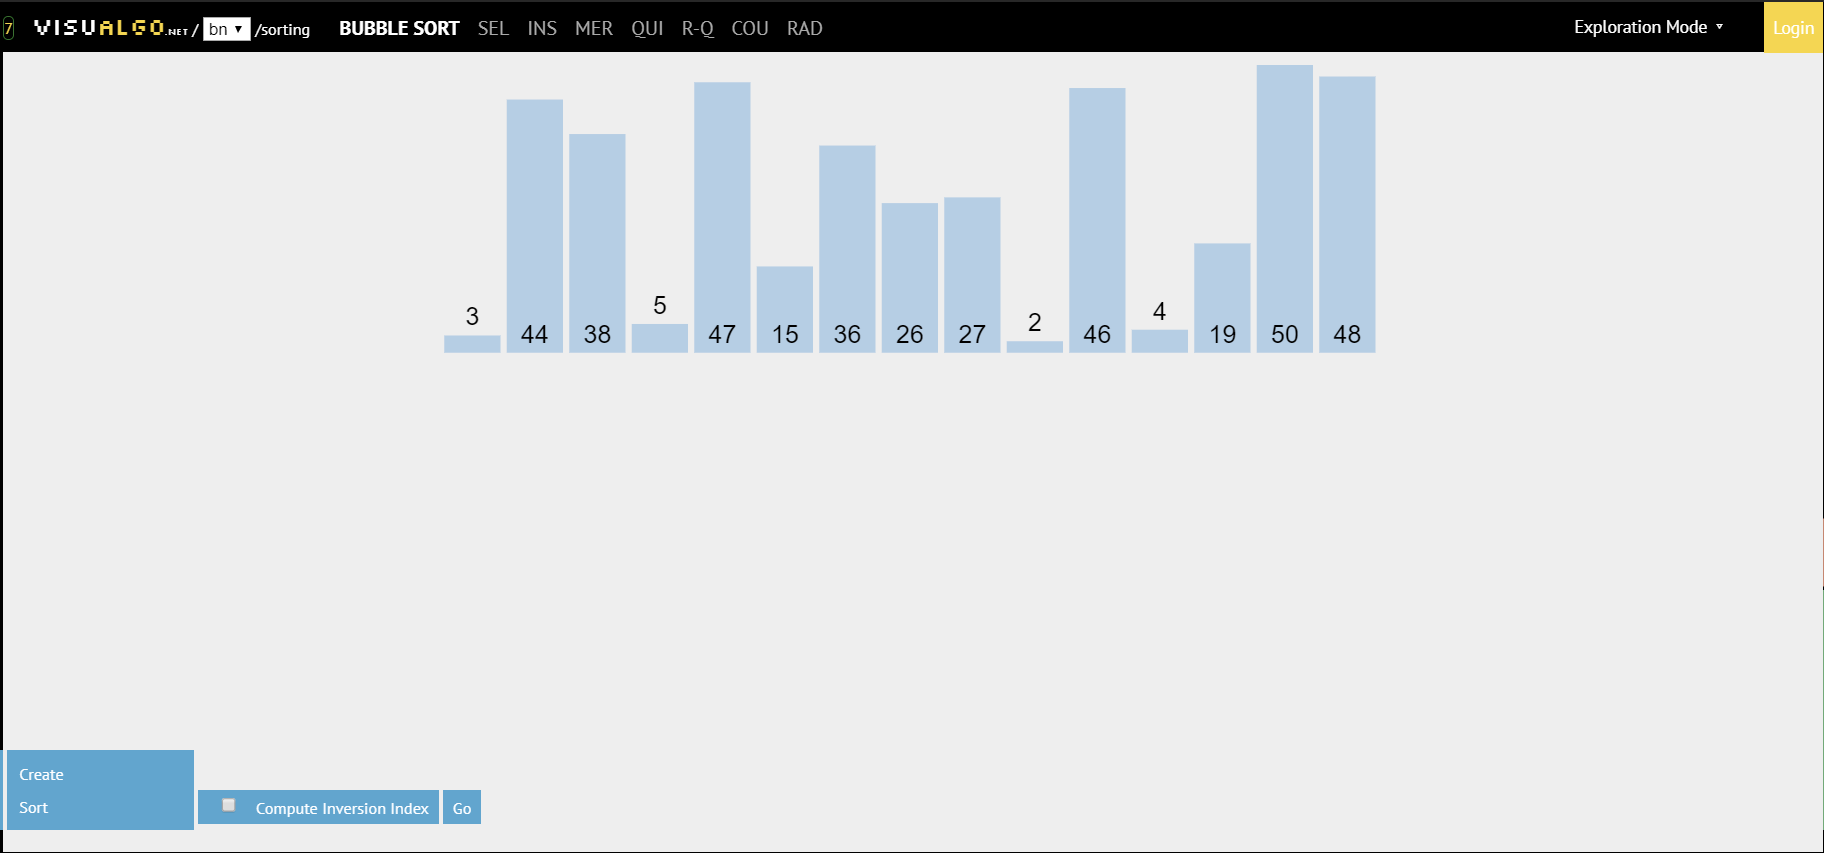
\includegraphics[width=12cm,height=12cm,keepaspectratio]{images/visalgosorting}
\end{center}
\newpage
Like VisuAlgo's sorting algorithms visualization component, the developed application allows the user to select different algorithms to visualize, the current elements being sorted are highlighted and swapped, and the user can enter their own data set to sort. I considered these features important for an application that would visualize sorting algorithms and, as such, implemented these in my own application.
\par
\bigskip
\subsection{Sorting Visualizer by Clement Mihailescu}
\begin{center}
    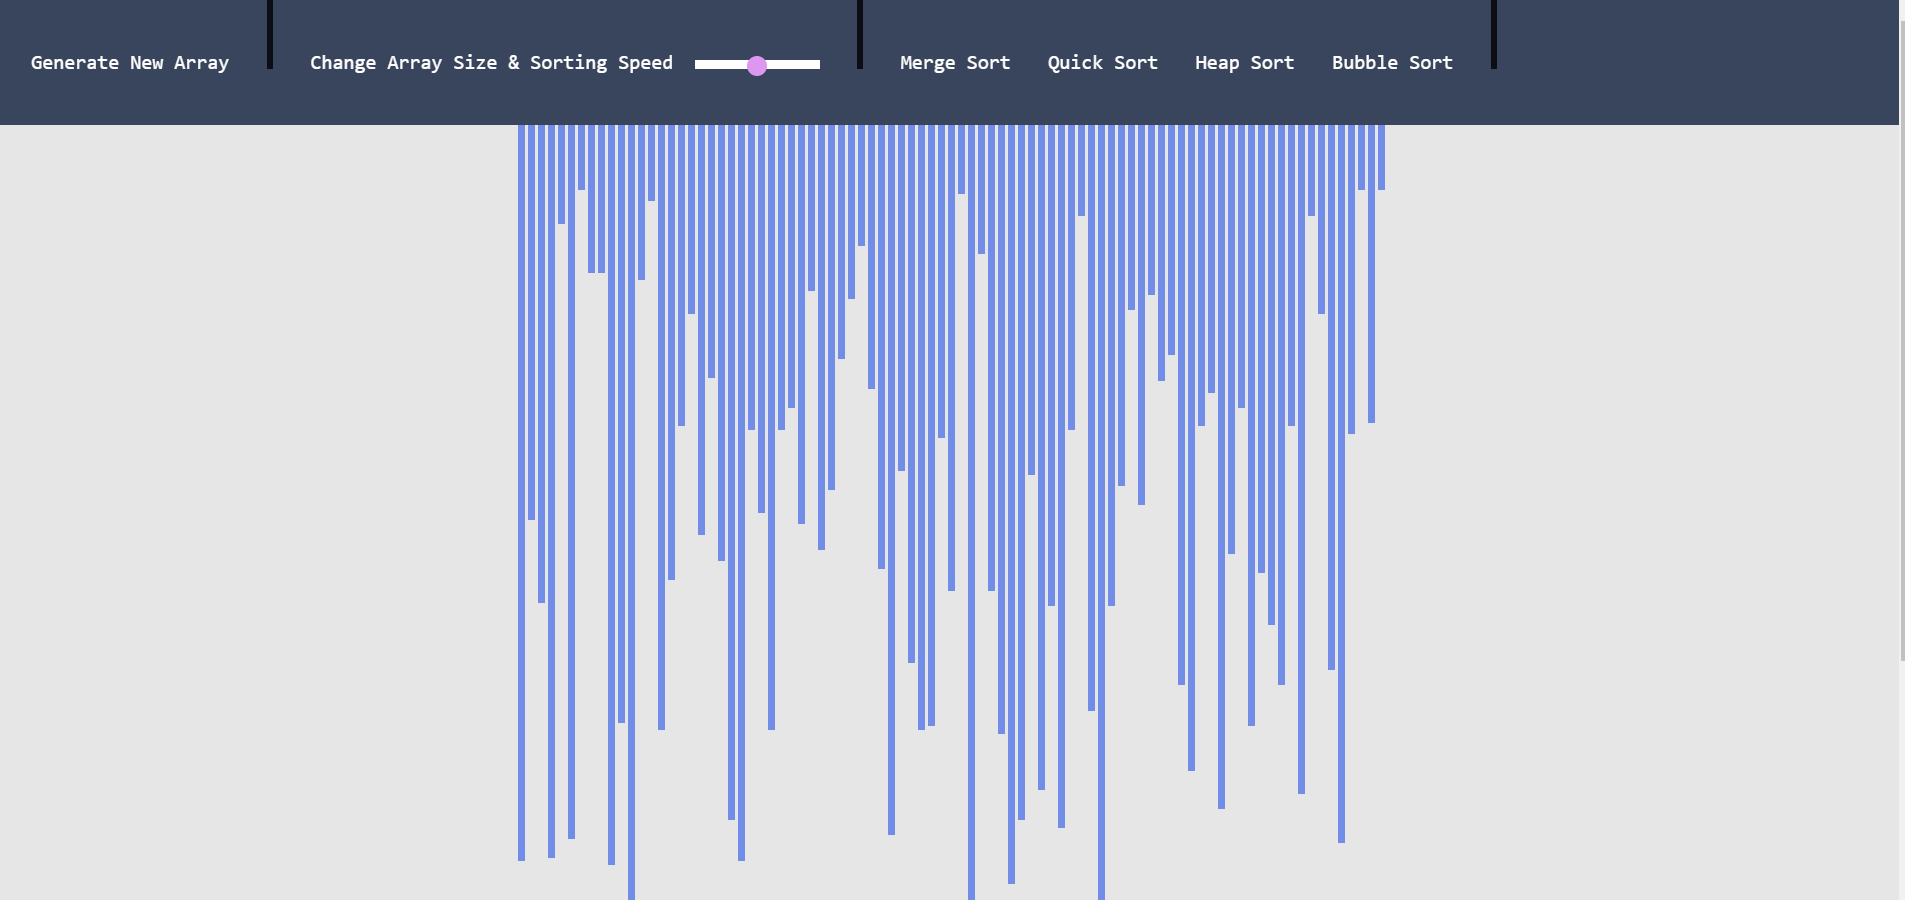
\includegraphics[width=12cm,height=12cm,keepaspectratio]{images/sortvisclement}
\end{center}
Like the other sorting visualizers, Clements Mihailescu's Sorting Visualizer \cite{sorting_1} follows a similar trend: allows the user to choose from several different sorting algorithms, generate a new array, and change the size of the array and the speed at which the array is sorting. Clements Mihailescu's Sorting Visualizer was developed in React, which was one of the main motivators behind using React for my application as, from research, it was found that React would be one of the best options for developing a visualization application.

\subsection{Comparison Sorting Visualization hosted by University of San Francisco}
\begin{center}
    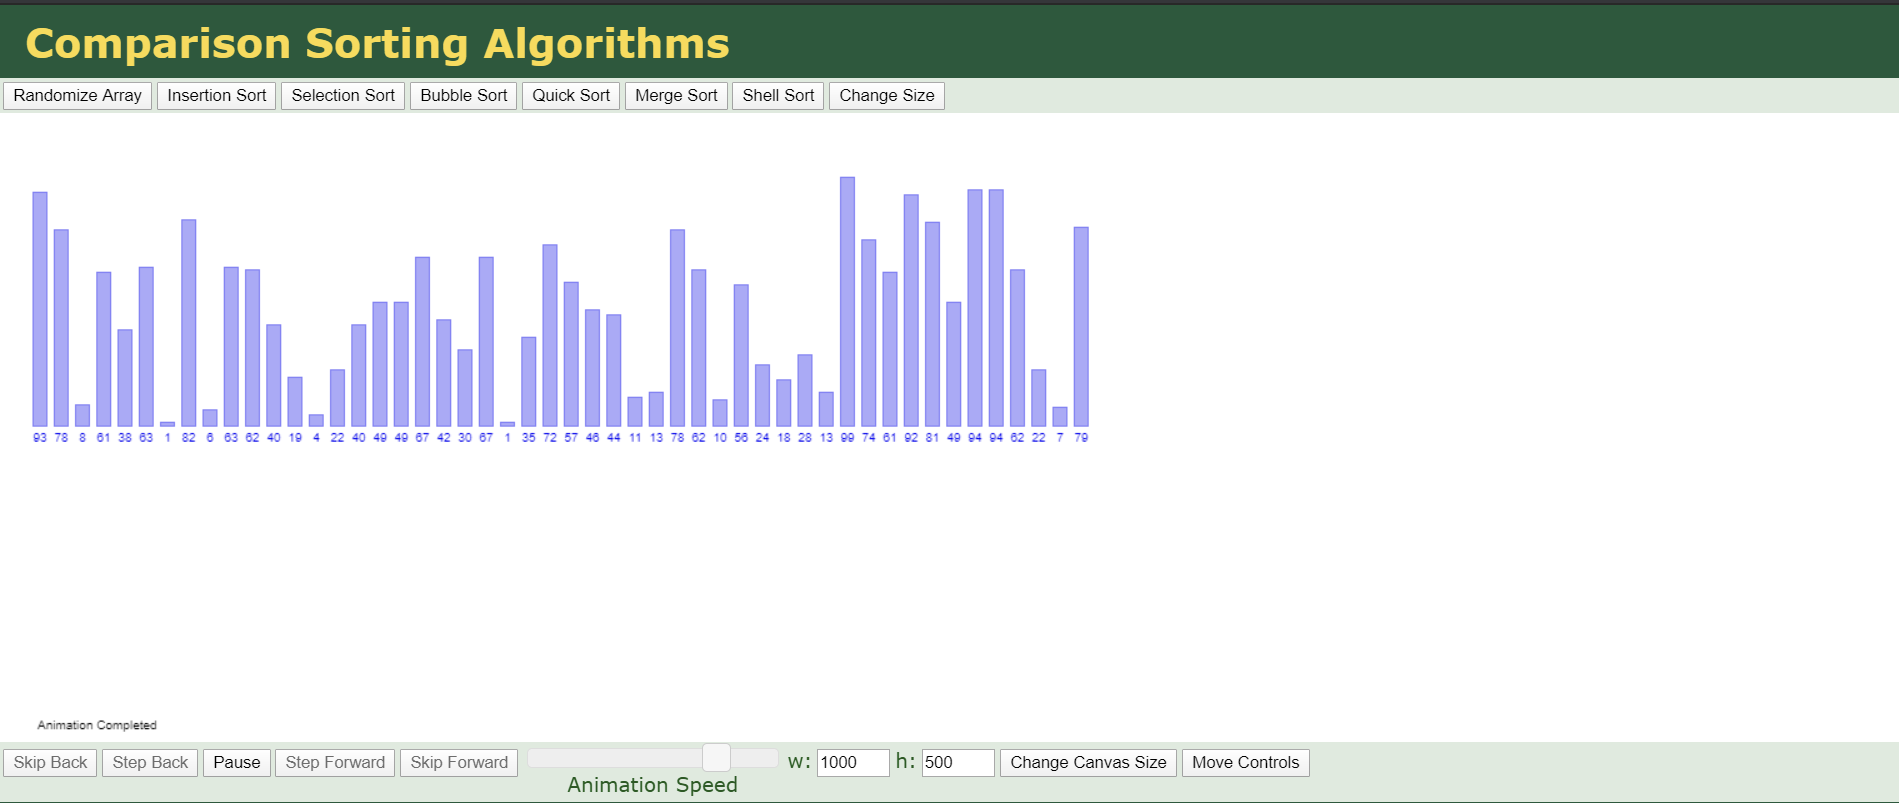
\includegraphics[width=12cm,height=12cm,keepaspectratio]{images/compsort}
\end{center}
Again, like the other sorting visualizer, the Comparison Sorting Visualization hosted by the University of San Francisco \cite{sorting_3} follows a similar trend. This application seemed to be a standard web application in HTML, JavaScript, and CSS. With this application, the user can randomize the array, select different algorithms to visualize, pause the sort, skip forward and back through the visualization, step back and forward through the sort, and change the size of the array of elements. Some of the features from this inspired features in my application, such as pausing the sort midway and randomizing the array multiple times before the user decides to sort it.

\newpage
\section{Software Development Methodology}
\begin{center}
    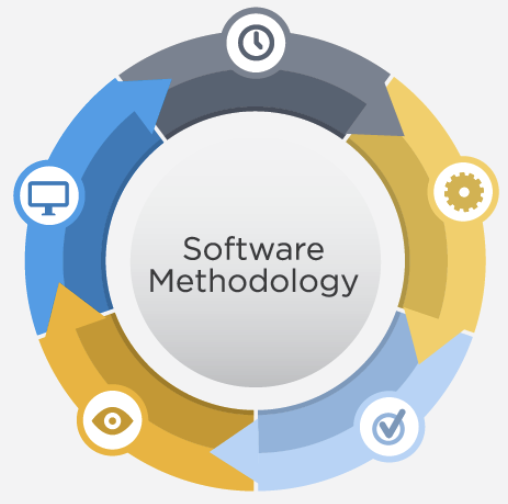
\includegraphics[width=8cm,height=3.3cm,keepaspectratio]{images/software_methodology}
    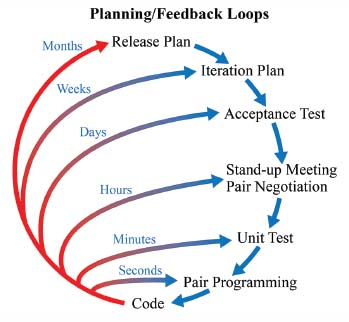
\includegraphics[width=8cm,height=3.3cm,keepaspectratio]{images/xp}
\end{center}
\par
The software development methodology that was used in this project was Extreme 
Programming (XP). Extreme Programming is a software development methodology 
designed to improve the quality of software and its ability to properly adapt to
the changing needs of the customer or client. While there was no customer or 
client for this project, this methodology was still applicable. 
\par
\medskip
\begin{center}
    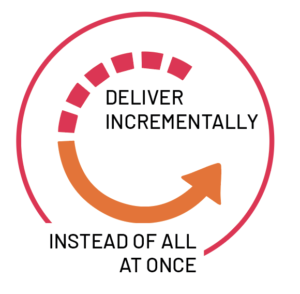
\includegraphics[width=8cm,height=3.3cm,keepaspectratio]{images/agile}
\end{center}
It is a form of Agile software development. The Agile methodology was developed 
as a response to growing frustrations with Waterfall and other highly 
structured, inflexible methodologies. This approach is designed to accommodate 
change and the need to produce software faster. Similar to other Agile methods 
of development, Extreme Programming aims to provide iterative and frequent small
releases throughout the project, allowing both team members and customers to 
examine and review the project’s progress throughout the entire SDLC (Software
Development Life Cycle). 
\par
\medskip
It became clear early on that the Agile methodology would be the most suitable 
methodology to use for this project as the Agile Methodology allows for 
incremental development, changing requirements, prototyping, and sustainable 
development. As there would be weekly meetings with the project supervisor, 
being able to show and discuss the progress of the project would be a bonus. 

\newpage
\section{Meetings}
Project meetings were held weekly for the duration of the project with the
project supervisor. The majority of the meetings consisted of:
\begin{itemize}
    \item Project progress updates.
    \item Feedback on progress.
    \item Planning of the next development iteration.
    \item Discussions on possible additional features that could be
    incorporated.
    \item Q&A on various project elements.
\end{itemize}
\par
\medskip
Initial project meetings were more focused on brainstorming possible projects
that could be developed. The first few weeks comprised of research, whereby 
possible projects ideas, appropriate technologies, and a project timeline was
developed. Next, the system design was designed and a feature timeline was discussed. After this, the project was implemented with weekly meetings used to review the current progress and state of the project each week. Throughout the development of the project, any changes and problems were discussed in the meetings, and solutions were examined to see how these challenges would be overcome.

\section{Development Tools}
\begin{center}
    
\includegraphics[width=8cm,height=3.3cm,keepaspectratio]{images/vscode}
\end{center}
The main Integrated Development Environment used throughout the project was 
Visual Studio Code. Visual Studio Code is a source-code editor developed by 
Microsoft for Windows, Linux and mac OS. It includes support for debugging, 
embedded Git control and GitHub, syntax highlighting, intelligent code 
completion, snippets, and code refactoring. 
\par
\bigskip
Visual Studio Code is based on Electron, a framework which is used to develop
Node.js applications for the desktop running on the Blink layout engine. Visual 
Studio Code is a source code editor that can be used with a variety of 
programming languages, including Java, JavaScript, Go, Node.js and C++.

Visual Studio Code was used throughout the development of the project as an obvious choice. Visual Studio Code provides support for many different types of files, which aids in development. It also has an in-built terminal which provides a detailed output and updates on project changes and output and feedback when the project is run. It also supports the installation of various different libraries and extensions through the command line or the built-in Marketplace. 

While certain IDEs are more suitable to certain languages (such as Eclipse being used to develop Java projects), Visual Studio Code is very suitable to developing web applications due to it's design. 


\section{Source Control}
\begin{center}
    
\includegraphics[width=8cm,height=3.3cm,keepaspectratio]{images/github}
\end{center}

Source control (or version control) is the practice of tracking and managing
changes to code. GitHub provides hosting for software development version
control using Git. Git is an open-source distributed source code management
system.

\subsubsection{Advantages}
There are a number of advantages to using Git:

\begin{itemize}
    \item \textbf{Distributed Development} - Git is a distributed version
    control system. Instead of a working copy, each developer gets their own 
    local repository, complete with a full history of commits. Having a full 
    local history makes Git fast, since it means you don’t need a network 
    connection to create commits, inspect previous versions of a file, or 
    perform diffs between commits. 
    \item \textbf{Faster Release Cycle} - As a result of feature branches,
    distributed development, pull requests, etc. is a faster release cycle. This
    facilitates an agile workflow, encouraging developers to share smaller 
    changes more frequently. This results in changes get pushed down the 
    development pipeline faster
\end{itemize}

\newpage
\subsubsection{Disadvantages}
Git is a very well-designed tool and, as such, has very few disadvantages:

\begin{itemize}
    \item \textbf{Pricing} - Some of GitHub features, as well as features on 
    other online repositories, are locked behind a SaaS paywall. If you have a 
    large team, this can add up fast. Those who already have a dedicated IT team
    and their own internal servers are often better off using their own internal
    git for cost reasons, but for most, the cost isn’t outrageous.
    \item \textbf{Security} - GitHub does offer private repositories, but this
    isn’t necessarily perfect for many. For high value intellectual property, 
    you’re putting all of this in the hands of GitHub as well as anyone who has 
    a login, which like many sites has had security breaches before and is 
    targeted constantly. In addition, some clients/employers will only allow 
    code on their own secure internal Git as a matter of policy.
\end{itemize}